\documentclass[aspectratio=169]{beamer}

\usepackage{amssymb,amsmath}
\usepackage{graphicx}
\usepackage{url}
\usepackage{color}
\usepackage{pagenote}[continuous,page]
\usepackage{relsize}		% For \smaller
\usepackage{url}			% For \url
\usepackage{epstopdf}	% Included EPS files automatically converted to PDF to include with pdflatex

%For MindMaps
% \usepackage{tikz}%
% \usetikzlibrary{mindmap,trees,arrows}%

%%% Color Definitions %%%%%%%%%%%%%%%%%%%%%%%%%%%%%%%%%%%%%%%%%%%%%%%%%%%%%%%%%
%\definecolor{bordercol}{RGB}{40,40,40}
%\definecolor{headercol1}{RGB}{186,215,230}
%\definecolor{headercol2}{RGB}{80,80,80}
%\definecolor{headerfontcol}{RGB}{0,0,0}
%\definecolor{boxcolor}{RGB}{186,215,230}

%%% Save space in lists. Use this after the opening of the list %%%%%%%%%%%%%%%%
%\newcommand{\compresslist}{
%	\setlength{\itemsep}{1pt}
%	\setlength{\parskip}{0pt}
%	\setlength{\parsep}{0pt}
%}

%\setbeameroption{show notes on top}

% You should run 'pdflatex' TWICE, because of TOC issues.

% Rename this file.  A common temptation for first-time slide makers
% is to name it something like ``my_talk.tex'' or
% ``john_doe_talk.tex'' or even ``discrete_math_seminar_talk.tex''.
% You really won't like any of these titles the second time you give a
% talk.  Try naming your tex file something more descriptive, like
% ``riemann_hypothesis_short_proof_talk.tex''.  Even better (in case
% you recycle 99% of a talk, but still want to change a little, and
% retain copies of each), how about
% ``riemann_hypothesis_short_proof_MIT-Colloquium.2000-01-01.tex''?

\mode<presentation>
{
  \usetheme{CambridgeUS}		% bem bacana - menu superior
  \usecolortheme{default}		% branco, azul clarinho
  \useoutertheme{default}
  \useinnertheme{circles}
  \setbeamercovered{invisible}
}

\beamertemplatenavigationsymbolsempty

%% Better looking blocks
\setbeamercolor{block title alerted}{use=structure,fg=black,bg=red!80!black}
\setbeamercolor{block body alerted}{use=structure,fg=black,bg=white!90!black}

\setbeamercolor{block title}{use=structure,fg=black,bg=blue!60!white}
\setbeamercolor{block body}{use=structure,fg=black,bg=white!90!black}

\usepackage[english]{babel}
\usepackage[latin1]{inputenc}
\usepackage{subfigure}

\usepackage{times}
\usepackage[T1]{fontenc}

%% makes the ppagenote command for figure references at the end.
\makepagenote
\renewcommand{\notenumintext}[1]{}
\newcommand{\ppagenote}[1]{\pagenote[Page \insertframenumber]{#1}}


\usepackage{tikz}
\usetikzlibrary{arrows,shapes}

\title[GB13624]{GB13624 - Maths for Computer Science}
\subtitle[]{Lecture 5 -- Graphs Part II}
\author[Claus Aranha]{Claus Aranha\\{\footnotesize caranha@cs.tsukuba.ac.jp}}
\institute[COINS]{College of Information Science}
\date[2020-11-04]{2020-11-04\\{\tiny Last updated \today}}

\tikzstyle{vertex}=[circle,fill=black!25,minimum size=10pt,inner sep=0pt]
\tikzstyle{blue vertex}=[circle,fill=blue!100,minimum size=10pt,inner sep=0pt]
\tikzstyle{red vertex}=[circle,fill=red!100,minimum size=10pt,inner sep=0pt]
\tikzstyle{yellow vertex}=[circle,fill=yellow!100,minimum size=10pt,inner sep=0pt]
\tikzstyle{edge} = [draw,thick,-]
\tikzstyle{pedge} = [draw,thick,.]
\tikzstyle{red edge} = [draw, thick,-,red!50]
\tikzstyle{black edge} = [draw, line width=2pt,-,black!20]
\tikzstyle{weight} = [font=\smaller]

\begin{document}

\begin{frame}
  \maketitle

  \begin{columns}
    \column{0.8\textwidth}
    {\smaller This course is based on Mathematics for Computer Science, Spring
    2015, by Albert Meyer and Adam Chlipala, Massachusetts Institute
    of Technology OpenCourseWare.}
    \column{0.2\textwidth}
    
\includegraphics[width=\textwidth]{../img/by-nc-sa}
  \end{columns}
\end{frame}

\begin{frame}{Graphs -- Lectures 4 and 5}
  \begin{columns}
    \column{0.5\textwidth}
    \begin{center}
      Lecture I: Chapter 9
    \end{center}
    \begin{itemize}
      \item Graphs and Relations
      \item Directed Graphs and Walks
      \item Scheduling and Partial Orders
    \end{itemize}

    \column{0.5\textwidth}
    \begin{center}
      Lecture II: Chapter 11
    \end{center}
    \begin{itemize}
    \item Using Isomorphism
    \item Coloring and Connectivity
    \item Spanning Trees
    \item Matching
    \end{itemize}
  \end{columns}
\end{frame}

\section{Graph Isomorphism}

\frame{
{Part 1: Graph Isomorphism}

\tableofcontents[currentsection,hideallsubsections, firstsection=1, sections={1-4}]
}

\begin{frame}{Directed Graphs and Simple Graphs}
  \begin{columns}[T]
    \column{0.5\textwidth}
    \begin{center}
      Directed Graph:\\

      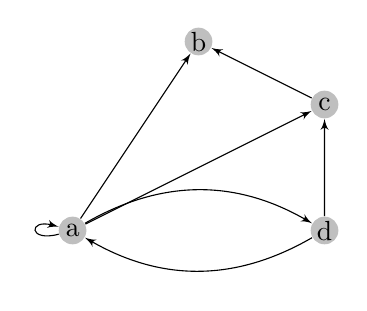
\begin{tikzpicture}[scale=.8,auto,swap]
        \tikzset{edge/.style = {->,>=latex'}}
        \node[vertex] (a) at (0,0) {a};
        \node[vertex] (b) at (2,3) {b};
        \node[vertex] (c) at (4,2) {c};
        \node[vertex] (d) at (4,0) {d};
        \draw[edge] (a) to (b);
        \draw[edge] (a) to (c);
        \draw[edge] (c) to (b);
        \draw[edge] (d) to (c);
        \draw[edge] (d) to[bend left] (a);
        \draw[edge] (a) to[bend left] (d);
        \draw[edge] (a) to[loop left] (a);
      \end{tikzpicture}
    \end{center}
    \column{0.5\textwidth}
    \begin{center}
      Simple Graph:\\

      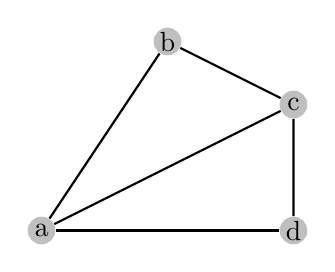
\begin{tikzpicture}[scale=.8,auto,swap]
        %\tikzset{edge/.style = {->,>=latex'}}
        \node[vertex] (a) at (0,0) {a};
        \node[vertex] (b) at (2,3) {b};
        \node[vertex] (c) at (4,2) {c};
        \node[vertex] (d) at (4,0) {d};
        \draw[edge] (a) to (b);
        \draw[edge] (a) to (c);
        \draw[edge] (c) to (b);
        \draw[edge] (d) to (c);
        \draw[edge] (d) to (a);
      \end{tikzpicture}

      \vspace{2em}
    \end{center}
    \begin{itemize}
    \item No double edges allowed;
    \item No self-loop allowed;
    \end{itemize}
  \end{columns}
\end{frame}

\begin{frame}{Simple Graphs}{Some definitions}
  A Simple Graph \structure{$G$} consists of:
  \begin{itemize}
  \item A \emph{non-empty} set \structure{$V$} of vertices;
  \item A set \structure{$E$} of edges so that:
    \begin{itemize}
    \item Each edge has \structure{two endpoints} in $V$:
      \hfill (\alert{not an {\bf start} and an {\bf end}})

      \bigskip
    \item The order of the vertices in an edge does not matter:
      \hfill $e_1 = \{v_1,v_2\} = \{v_2, v_1\}$

      \bigskip
    \item Two vertices with an edge between them are
      \structure{adjacent}

      \bigskip
    \item An edge that connects two vertices is \structure{incident}
      to them.
      \hfill Ex: $e_1$ is \structure{incident} to $v_1$ and $v_2$
    \end{itemize}
  \end{itemize}
\end{frame}

\begin{frame}{Vertice Degrees}

    The \structure{degree} of a vertex is the \structure{number of
      incident edges}.

    \begin{center}
      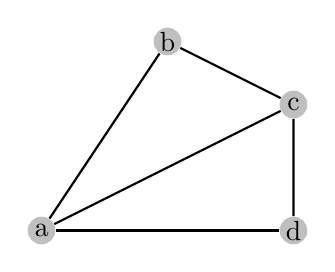
\begin{tikzpicture}[scale=.8,auto,swap]
        %\tikzset{edge/.style = {->,>=latex'}}
        \node[vertex] (a) at (0,0) {a};
        \node[vertex] (b) at (2,3) {b};
        \node[vertex] (c) at (4,2) {c};
        \node[vertex] (d) at (4,0) {d};
        \draw[edge] (a) to (b);
        \draw[edge] (a) to (c);
        \draw[edge] (c) to (b);
        \draw[edge] (d) to (c);
        \draw[edge] (d) to (a);
      \end{tikzpicture}

      deg(a) = 3 \hspace{1cm} deg(d) = 2
    \end{center}

    \hfill

    \alert{Quiz:} Can you build a graph with following vertice degrees?
    \begin{itemize}
    \item 3, 2, 2, 1 (four vertices)
    \item 3, 2, 2, 2 (four vertices)
    \end{itemize}
\end{frame}

\begin{frame}{Verdice Degrees}{The Handshaking Lemma}

  {\bf Lemma:} The sum of vertice degrees in a graph is 2x the number of edges.
  \begin{equation}
    2|E| = \sum_{v\in V} \text{deg}(v)
  \end{equation}

  \begin{proof}
    \begin{itemize}
      \item Every edge in a graph connects two vertices;
      \item If we begin with a graph with 0 edges, for every edge $(v_i,v_j)$ that we add to the graph, we add 2 vertice degrees (one for $v_i$, one for $v_j$).
      \item So the total of vertices is 2 times the total of edges.
    \end{itemize}
  \end{proof}\bigskip

  Because of the lemma, it is impossible to make a graph with vertice degrees 3, 2, 2, 2.
\end{frame}

\subsection{Isomorphism}

\begin{frame}{Review: Isomorphism in graphs}{Remember: an isomorphism is an edge preserving bijection}
    \begin{columns}
      \column{0.5\textwidth}
      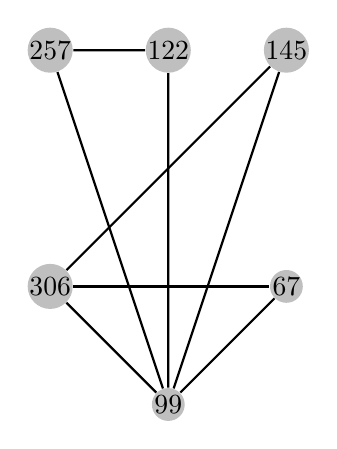
\begin{tikzpicture}[scale=1.5,auto,swap]
        %\tikzset{edge/.style = {->,>=latex'}}
        \node[vertex] (257) at (0,2) {257};
        \node[vertex] (122) at (1,2) {122};
        \node[vertex] (145) at (2,2) {145};
        \node[vertex] (306) at (0,0) {306};
        \node[vertex] (67) at (2,0) {67};
        \node[vertex] (99) at (1,-1) {99};
        \draw[edge] (257) to (122);
        \draw[edge] (257) to (99);
        \draw[edge] (122) to (99);
        \draw[edge] (306) to (99);
        \draw[edge] (67) to (99);
        \draw[edge] (306) to (67);
        \draw[edge] (306) to (145);
        \draw[edge] (145) to (99);
      \end{tikzpicture}

      \column{0.5\textwidth}
      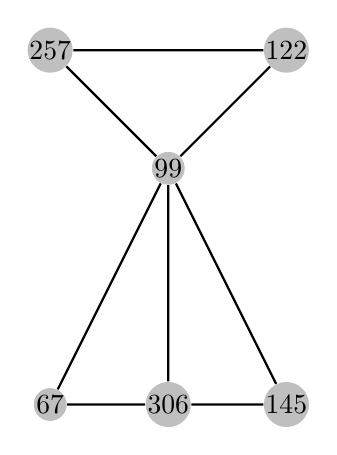
\begin{tikzpicture}[scale=1.5,auto,swap]
        %\tikzset{edge/.style = {->,>=latex'}}
        \node[vertex] (257) at (0,2) {257};
        \node[vertex] (122) at (2,2) {122};
        \node[vertex] (145) at (2,-1) {145};
        \node[vertex] (306) at (1,-1) {306};
        \node[vertex] (67) at (0,-1) {67};
        \node[vertex] (99) at (1,1) {99};
        \draw[edge] (257) to (122);
        \draw[edge] (257) to (99);
        \draw[edge] (122) to (99);
        \draw[edge] (306) to (99);
        \draw[edge] (67) to (99);
        \draw[edge] (306) to (67);
        \draw[edge] (306) to (145);
        \draw[edge] (145) to (99);
      \end{tikzpicture}

    \end{columns}\bigskip

    The left and the right are \structure{the same graph}, but with different positions for the vertices.
\end{frame}

\begin{frame}{Review: Isomorphism in graphs}{Remember: Isomorphism is an edge preserving vertex bijection}
    \begin{columns}
      \column{0.5\textwidth}
      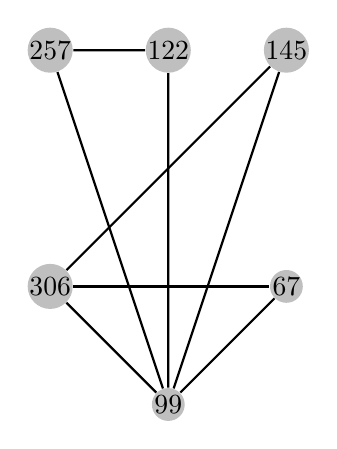
\begin{tikzpicture}[scale=1.5,auto,swap]
        %\tikzset{edge/.style = {->,>=latex'}}
        \node[vertex] (257) at (0,2) {257};
        \node[vertex] (122) at (1,2) {122};
        \node[vertex] (145) at (2,2) {145};
        \node[vertex] (306) at (0,0) {306};
        \node[vertex] (67) at (2,0) {67};
        \node[vertex] (99) at (1,-1) {99};
        \draw[edge] (257) to (122);
        \draw[edge] (257) to (99);
        \draw[edge] (122) to (99);
        \draw[edge] (306) to (99);
        \draw[edge] (67) to (99);
        \draw[edge] (306) to (67);
        \draw[edge] (306) to (145);
        \draw[edge] (145) to (99);
      \end{tikzpicture}

      \column{0.5\textwidth}
      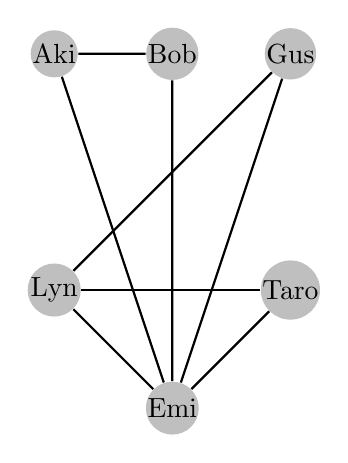
\begin{tikzpicture}[scale=1.5,auto,swap]
        %\tikzset{edge/.style = {->,>=latex'}}
        \node[vertex] (257) at (0,2) {Aki};
        \node[vertex] (122) at (1,2) {Bob};
        \node[vertex] (145) at (2,2) {Gus};
        \node[vertex] (306) at (0,0) {Lyn};
        \node[vertex] (67) at (2,0) {Taro};
        \node[vertex] (99) at (1,-1) {Emi};
        \draw[edge] (257) to (122);
        \draw[edge] (257) to (99);
        \draw[edge] (122) to (99);
        \draw[edge] (306) to (99);
        \draw[edge] (67) to (99);
        \draw[edge] (306) to (67);
        \draw[edge] (306) to (145);
        \draw[edge] (145) to (99);
      \end{tikzpicture}

    \end{columns}\bigskip

    The left and the right are \structure{the same graph}, but with different {\bf labels} for the vertices.
\end{frame}

\begin{frame}{Isomorphism}

    \begin{itemize}
    \item Graph Isomorphism is determined solely by the edges between vertices;\bigskip

    \item Two graphs with the same edge connections are \structure{isomorphic};\bigskip

    \item Formally, wwo graphs are isomorphic if there is an \structure{Edge Preserving Matching Relation} between their vertices;\bigskip
    \end{itemize}
\end{frame}

\begin{frame}{Isomorphism}{Are these graphs Isomorphic?}

    \begin{columns}
      \column{0.5\textwidth}
      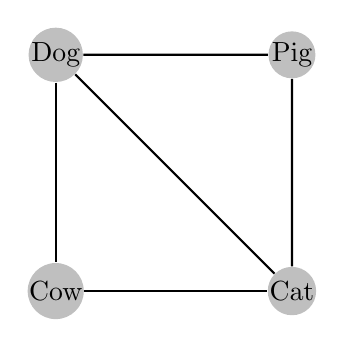
\begin{tikzpicture}[scale=1.5,auto,swap]
        %\tikzset{edge/.style = {->,>=latex'}}
        \node[vertex] (a) at (0,0) {Cow};
        \node[vertex] (b) at (2,0) {Cat};
        \node[vertex] (c) at (0,2) {Dog};
        \node[vertex] (d) at (2,2) {Pig};
        \draw[edge] (a) to (b);
        \draw[edge] (b) to (d);
        \draw[edge] (d) to (c);
        \draw[edge] (c) to (a);
        \draw[edge] (c) to (b);
      \end{tikzpicture}
      \column{0.5\textwidth}
      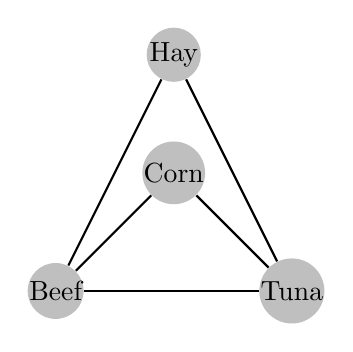
\begin{tikzpicture}[scale=1.5,auto,swap]
        %\tikzset{edge/.style = {->,>=latex'}}
        \node[vertex] (a) at (1,2) {Hay};
        \node[vertex] (b) at (2,0) {Tuna};
        \node[vertex] (c) at (0,0) {Beef};
        \node[vertex] (d) at (1,1) {Corn};
        \draw[edge] (a) to (b);
        \draw[edge] (b) to (d);
        \draw[edge] (d) to (c);
        \draw[edge] (c) to (a);
        \draw[edge] (c) to (b);
      \end{tikzpicture}
    \end{columns}\bigskip

    Edge Preserving Bijection:\\
    f(dog) = Beef; \hspace{2cm} f(cow) = Hay\\
    f(cat) = Tuna; \hspace{2cm} f(pig) = Corn
\end{frame}

\begin{frame}{Isomorphism}{Are THESE graphics Isomorphic? (2)}

  \begin{center}
    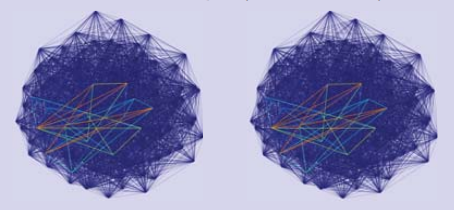
\includegraphics[width=0.8\textwidth]{../img/isomorphism}
    \pagenote{Isomorphism image from MIT OCW materials}
  \end{center}
\end{frame}

\begin{frame}{Graph Isomorphism}{Edge Preserving Bijection}

    $G_1$ \structure{isomorphic} to $G_2$ means that $\exists$
    Edge Preserving Vertex Matching:
    \begin{equation*}
      \exists f:V_1 \rightarrow V_2,
      (u,v) \in E_1 \iff (f(u),f(v)) \in E_2
    \end{equation*}\bigskip

    It is easy to quickly identify {\bf \alert{non-isomorphic}} graphs:
    \begin{itemize}
    \item Not the same number of vertices;
    \item Not the same number of edges;
    \item Not the same degree distribution;
    \item Differences in Paths, Distances, etc...
    \end{itemize}
\end{frame}

\begin{frame}{How to find Graph Isomorphism?}
    \begin{itemize}
      \item Finding the bijection is very hard:
      \begin{itemize}
        \item Total Number of possible bijections: permutation on $|V|$
        % TODO: add an example here about how to find bijections by enumerating the permutations
      \end{itemize}\bigskip

    \item If the graph is "small", can check the permutations by hand;\bigskip

    \item If the graph is "large", create random matchings $f: V_1 \rightarrow V_2$, and check:
      \begin{itemize}
        \item Quickly prune matchings that are {\bf not} isomorphic:
        \item Vertices in the bijection must have the same degree. (ex: a vertice with edge 4 must match to another vertice with edge 4)
        \item \emph{Adjacent vertices} must match degree as well. (ex: A vertice with degree 3, and neighbors with degree 4, 2, 1)
      \end{itemize}
    \end{itemize}
\end{frame}

\begin{frame}{How to find Graph Isomorphism?}

  Finding an isomorphism for two graphs is a very expensive, and important, problem. In theory, there is no algorithm that is better than just checking every possible bijection.

  \begin{center}
    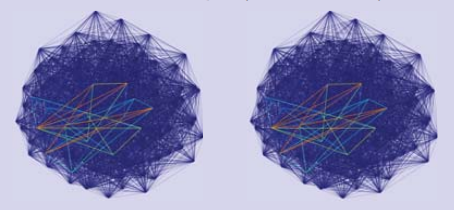
\includegraphics[width=0.8\textwidth]{../img/isomorphism}
    \pagenote{Isomorphism image from MIT OCW materials}
  \end{center}
\end{frame}

% TODO: Add some quizzes from the website

\section{Coloring}

\frame{
{Part 2: Graph Isomorphism}

\tableofcontents[currentsection,hideallsubsections, firstsection=1, sections={1-4}]
}


\begin{frame}{Graph Coloring: Airplanes and boarding gates}

  Graph coloring is a problem with several applications, such as \structure{scheduling problems}. Let's look at Gate scheduling:\bigskip

    {\bf Example}:
    \begin{itemize}
    \item Every flight requires a \structure{gate} for embark/disembark;
    \item Sometimes flight times overlap, so multiple gates are necessary;
    \item How many gates do we need to satisfy a flight schedule?
    \end{itemize}

  \hfill 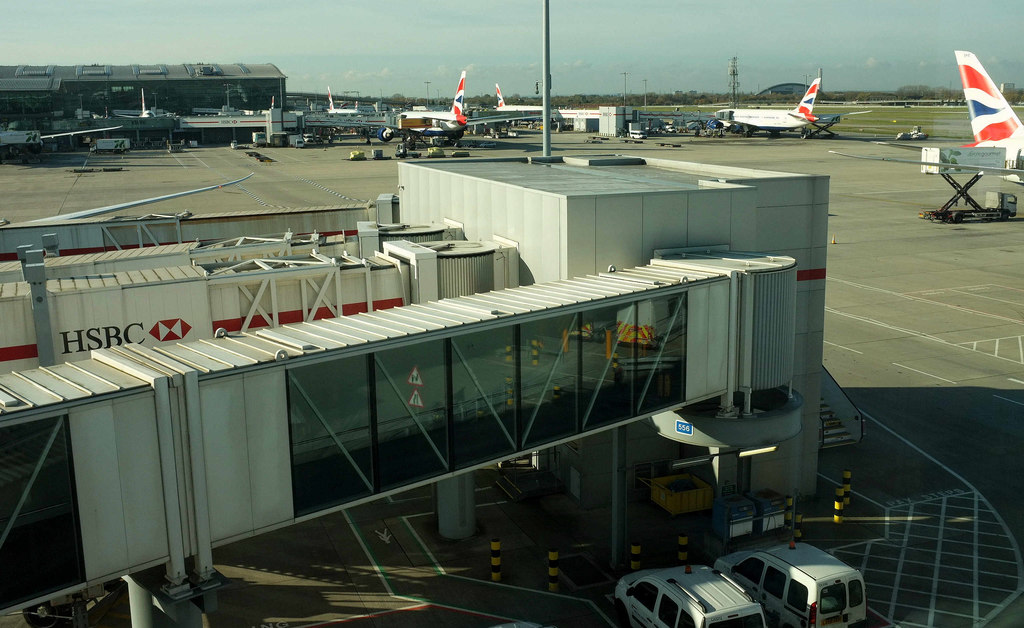
\includegraphics[width=0.5\textwidth]{../img/airgate}

\end{frame}

\begin{frame}{Boarding Gate Scheduling Graph}
  Let's define a \structure{Gate Scheduling Graph}, where each flight is a vertice, and an edge indicates that \alert{two flights are on the ground at the same time}.

    \begin{columns}[T]
      \column{0.6\textwidth}
      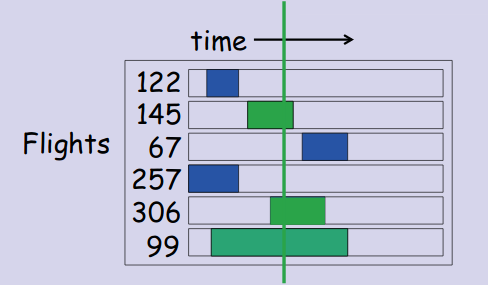
\includegraphics[width=1\textwidth]{../img/gatetable}
      \column{0.4\textwidth}
      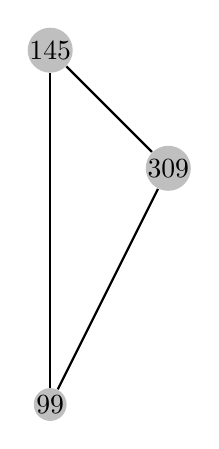
\begin{tikzpicture}[scale=1.5,auto,swap]
        %\tikzset{edge/.style = {->,>=latex'}}
        \node[vertex] (a) at (0,3) {145};
        \node[vertex] (b) at (1,2) {309};
        \node[vertex] (c) at (0,0) {99};
        \draw[edge] (a) to (b);
        \draw[edge] (b) to (c);
        \draw[edge] (c) to (a);
      \end{tikzpicture}

    \end{columns}
\end{frame}

\begin{frame}{Gate Scheduling Graph and Coloring}
    \begin{columns}
      \column{0.5\textwidth}
      \begin{center}
      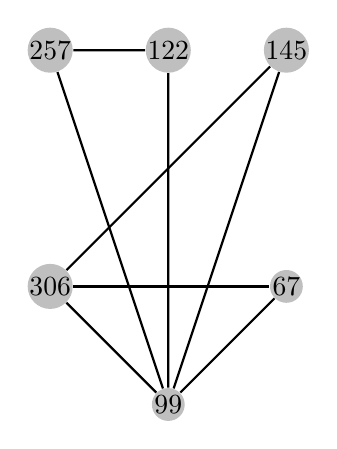
\begin{tikzpicture}[scale=1.5,auto,swap]
        %\tikzset{edge/.style = {->,>=latex'}}
        \node[vertex] (257) at (0,2) {257};
        \node[vertex] (122) at (1,2) {122};
        \node[vertex] (145) at (2,2) {145};
        \node[vertex] (306) at (0,0) {306};
        \node[vertex] (67) at (2,0) {67};
        \node[vertex] (99) at (1,-1) {99};
        \draw[edge] (257) to (122);
        \draw[edge] (257) to (99);
        \draw[edge] (122) to (99);
        \draw[edge] (306) to (99);
        \draw[edge] (67) to (99);
        \draw[edge] (306) to (67);
        \draw[edge] (306) to (145);
        \draw[edge] (145) to (99);
      \end{tikzpicture}
    \end{center}
      \column{0.5\textwidth}
      \begin{itemize}
        \item If each flight is a vertice, and each edge is a conflict, we can use \structure{graph coloring} to solve the problem.
        \item Each color is a new gate.
        \item If two vertices have an edge between them, the flights are \alert{in conflict}, and their colors must be different.
        \item The minimum number of colors to color all vertices is the same as the minimum number of boarding gates.
      \end{itemize}
    \end{columns}
\end{frame}


\begin{frame}{Gate Scheduling Graph and Coloring}
    \begin{columns}
      \column{0.5\textwidth}
      \begin{center}
      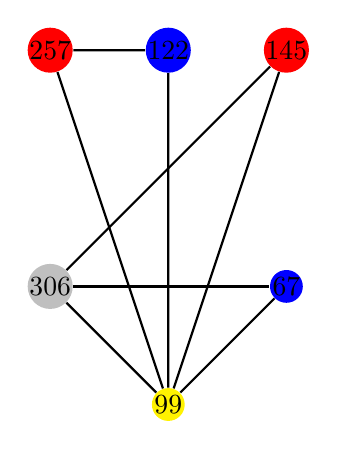
\begin{tikzpicture}[scale=1.5,auto,swap]
        %\tikzset{edge/.style = {->,>=latex'}}
        \node[red vertex] (257) at (0,2) {257};
        \node[blue vertex] (122) at (1,2) {122};
        \node[red vertex] (145) at (2,2) {145};
        \node[vertex] (306) at (0,0) {306};
        \node[blue vertex] (67) at (2,0) {67};
        \node[yellow vertex] (99) at (1,-1) {99};
        \draw[edge] (257) to (122);
        \draw[edge] (257) to (99);
        \draw[edge] (122) to (99);
        \draw[edge] (306) to (99);
        \draw[edge] (67) to (99);
        \draw[edge] (306) to (67);
        \draw[edge] (306) to (145);
        \draw[edge] (145) to (99);
      \end{tikzpicture}
    \end{center}
      \column{0.5\textwidth}
      \begin{itemize}
      \item We select colors for each vertex so that no adjacent
        vertex has the same color.

        \bigskip

      \item Each color = One new Gate

        \bigskip

      \item Final gate assignment:
        \begin{itemize}
        \item Blue Gate: Flight 122 and 67
        \item Red Gate: Flight 145 and 257
        \item Yellow Gate: Flight 99
        \item Gray Gate: Flight 306
        \end{itemize}

        \bigskip

      \item Can you find a better coloring using
        only \alert{3 gates}?
      \end{itemize}
    \end{columns}
\end{frame}

\begin{frame}{More Graph Coloring Problems}
    \begin{columns}
      \column{0.5\textwidth}
      \begin{itemize}
      \item \structure{Allocate classrooms} for courses.\\
        Some courses can be \alert{at the same time}.
        \medskip

      \item \structure{Allocate cages} for animals.
        Some animals \alert{can't live in the same cage}.
        \medskip

      \item \structure{Different Frequencies} for radio stations.
        Some frequencies \alert{interfere with each other}
        \medskip

      \item Color a map so that it look pretty!
      \end{itemize}

      \column{0.5\textwidth}
      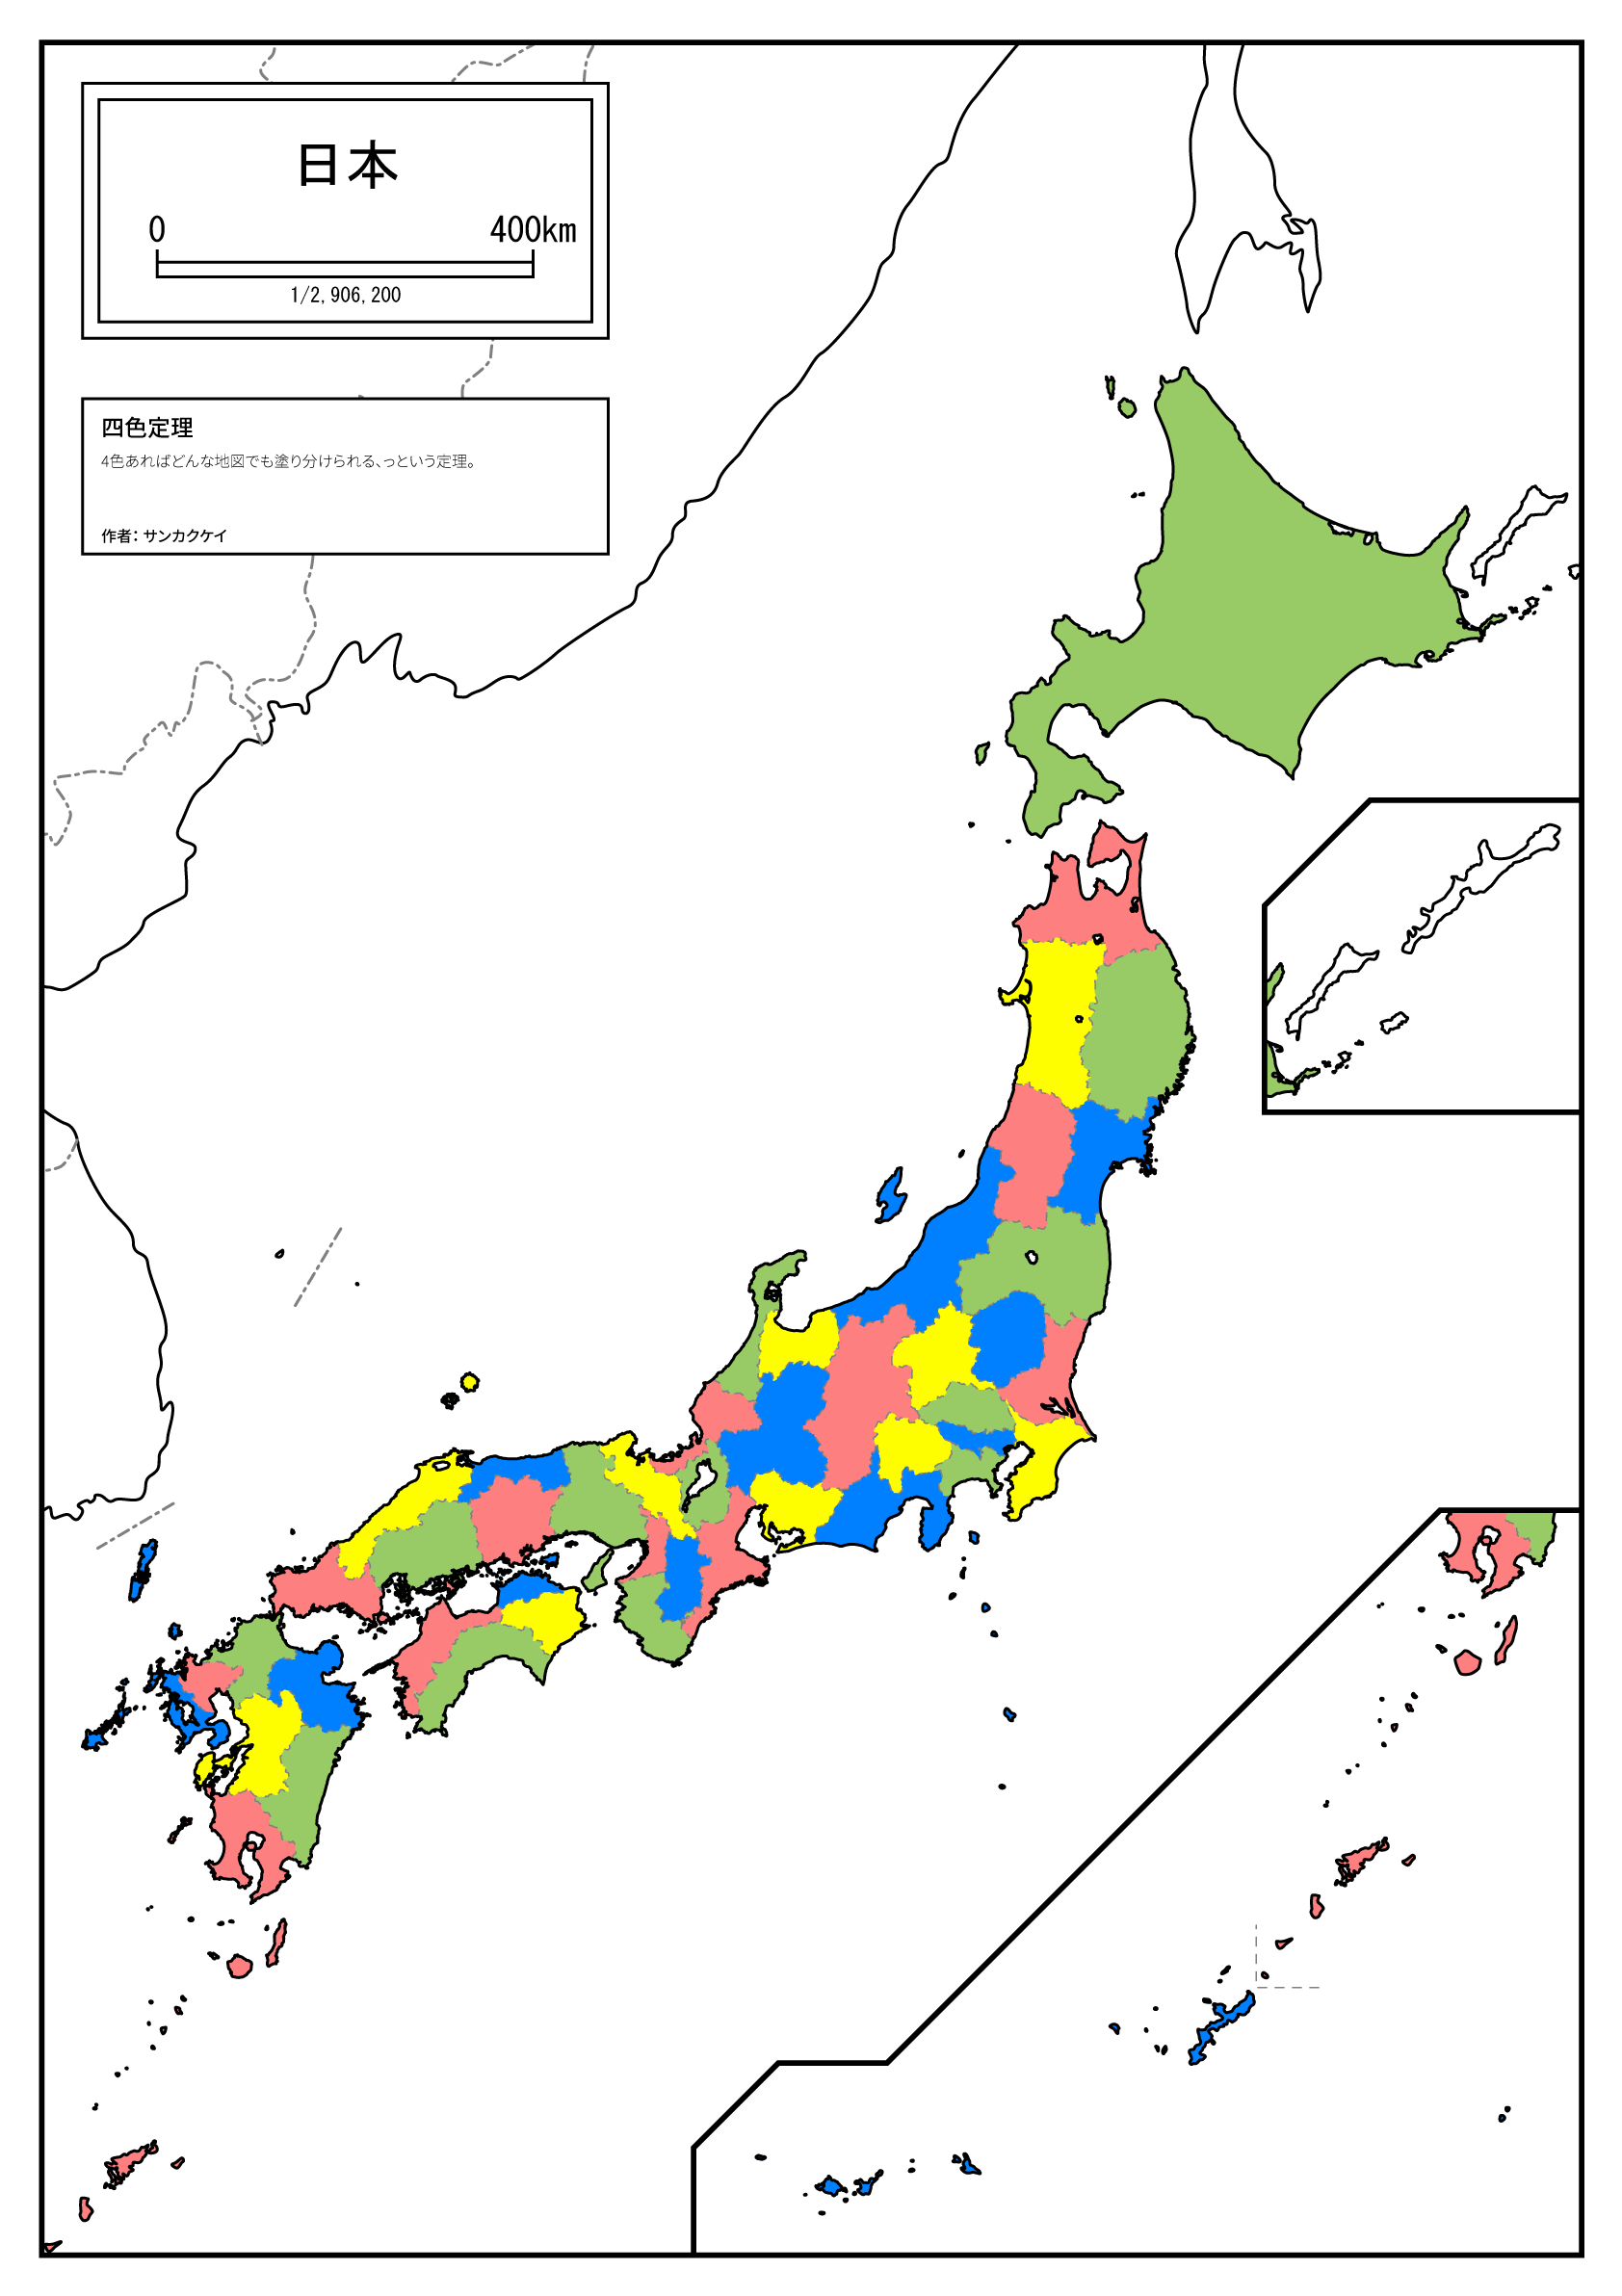
\includegraphics[height=.8\textheight]{../img/japan4color}
    \end{columns}
\end{frame}

\begin{frame}{Vertex Coloring and Face Coloring}

    \begin{center}
      Graphs (Vertices) to Maps (Faces) are equivalent when coloring!\\
      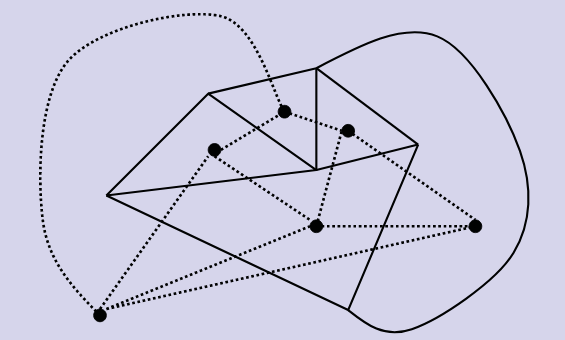
\includegraphics[width=0.5\textwidth]{../img/facecolor}
    \end{center}

    {\bf Theorem:} Maps can always be colored with 4 colors
    \begin{itemize}
    \item 1970: ``Proof'' with computers (automatically checks 1000's of maps)
    \item 1990: Better mathematical proof. (still needs programmed testing)
    \end{itemize}
\end{frame}

\begin{frame}{Chromatic Number}
    The Chromatic Number $\chi(G)$ is the \structure{minimum} number of
    colors needed for a graph $G$.

    {\bf Examples:} There are several rules for certain kinds of graphs:

    \begin{itemize}
    \item Cycle Graphs: $\chi(C_{\text{even}}) = 2$, $\chi(C_{\text{odd}}) = 3$\\
      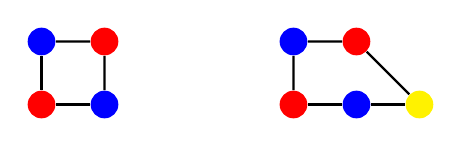
\begin{tikzpicture}[scale=.8,auto,swap]
        %\tikzset{edge/.style = {->,>=latex'}}
        \node[red vertex] (a) at (0,0) {};
        \node[blue vertex] (b) at (1,0) {};
        \node[red vertex] (c) at (1,1) {};
        \node[blue vertex] (d) at (0,1) {};
        \draw[edge] (a) to (b);
        \draw[edge] (b) to (c);
        \draw[edge] (c) to (d);
        \draw[edge] (d) to (a);
        \node[red vertex] (a1) at (4,0) {};
        \node[blue vertex] (b1) at (5,0) {};
        \node[red vertex] (c1) at (5,1) {};
        \node[blue vertex] (d1) at (4,1) {};
        \node[yellow vertex] (e1) at (6,0) {};
        \draw[edge] (a1) to (b1);
        \draw[edge] (b1) to (e1);
        \draw[edge] (e1) to (c1);
        \draw[edge] (c1) to (d1);
        \draw[edge] (d1) to (a1);
      \end{tikzpicture}

    \item Complete Graph with $n$ vertices: $\chi(K_n) = n$\\
      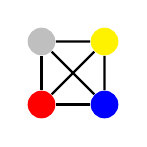
\begin{tikzpicture}[scale=.8,auto,swap]
        %\tikzset{edge/.style = {->,>=latex'}}
        \node[red vertex] (a) at (0,0) {};
        \node[blue vertex] (b) at (1,0) {};
        \node[yellow vertex] (c) at (1,1) {};
        \node[vertex] (d) at (0,1) {};
        \draw[edge] (a) to (b);
        \draw[edge] (b) to (c);
        \draw[edge] (c) to (d);
        \draw[edge] (d) to (a);
        \draw[edge] (a) to (c);
        \draw[edge] (d) to (b);
      \end{tikzpicture}

    \item Wheel Graph: $\chi(W_{\text{odd}}) = 4, \chi(W_{\text{even}} = 3)$
      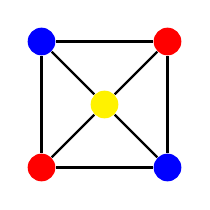
\begin{tikzpicture}[scale=.8,auto,swap]
        %\tikzset{edge/.style = {->,>=latex'}}
        \node[red vertex] (a) at (0,0) {};
        \node[blue vertex] (b) at (2,0) {};
        \node[red vertex] (c) at (2,2) {};
        \node[blue vertex] (d) at (0,2) {};
        \node[yellow vertex] (e) at (1,1) {};
        \draw[edge] (a) to (b);
        \draw[edge] (b) to (c);
        \draw[edge] (c) to (d);
        \draw[edge] (d) to (a);
        \draw[edge] (a) to (e);
        \draw[edge] (b) to (e);
        \draw[edge] (c) to (e);
        \draw[edge] (d) to (e);
      \end{tikzpicture}
    \end{itemize}
\end{frame}

\begin{frame}{Bounding Chromatic Numbers}{What is the maximum Chromatic Number?}

    \begin{itemize}
    \item If all vertex degrees are $\leq k \implies \chi(G) \leq k+1$\\
      \hfill (Proof by Greedy coloring algorithm).

      \bigskip

    \item Is a graph 2-colorable?\\
      \hfill ({\bf easy} to check: do a Breath First Search and mark as you go)\bigskip

    \item Is a graph 3-colorable?\\
      \hfill ({\bf very hard} to check: NP complete!)\bigskip

    \item Is $\chi(G) = k$?\\
      \hfill (in theory not harder than 3 color, harder in practice).

    \end{itemize}
\end{frame}

\subsection{Connectivity}

\begin{frame}{Connectivity}{Definition}

    \begin{itemize}
    \item Two vertices are \structure{connected} {\bf iff} there is a \structure{path} between the two.\bigskip

    \item Every vertice is connected to itself. (even if it does not have a self-edge)\bigskip

    \item A whole \structure{graph} is \structure{connected} if every vertice is connected to each other.
    \end{itemize}\bigskip

    \begin{center}
      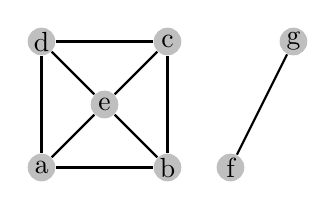
\begin{tikzpicture}[scale=.8,auto,swap]
        %\tikzset{edge/.style = {->,>=latex'}}
        \node[vertex] (a) at (0,0) {a};
        \node[vertex] (b) at (2,0) {b};
        \node[vertex] (c) at (2,2) {c};
        \node[vertex] (d) at (0,2) {d};
        \node[vertex] (e) at (1,1) {e};
        \node[vertex] (f) at (3,0) {f};
        \node[vertex] (g) at (4,2) {g};
        \draw[edge] (a) to (b);
        \draw[edge] (b) to (c);
        \draw[edge] (c) to (d);
        \draw[edge] (d) to (a);
        \draw[edge] (a) to (e);
        \draw[edge] (b) to (e);
        \draw[edge] (c) to (e);
        \draw[edge] (d) to (e);
        \draw[edge] (f) to (g);
      \end{tikzpicture}
    \end{center}
\end{frame}

\begin{frame}{Connected Components}{Vertex Connectivity}

    \begin{center}
      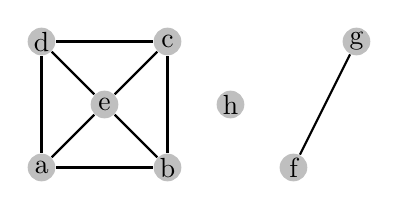
\begin{tikzpicture}[scale=.8,auto,swap]
        %\tikzset{edge/.style = {->,>=latex'}}
        \node[vertex] (a) at (0,0) {a};
        \node[vertex] (b) at (2,0) {b};
        \node[vertex] (c) at (2,2) {c};
        \node[vertex] (d) at (0,2) {d};
        \node[vertex] (e) at (1,1) {e};
        \node[vertex] (f) at (4,0) {f};
        \node[vertex] (g) at (5,2) {g};
        \node[vertex] (h) at (3,1) {h};
        \draw[edge] (a) to (b);
        \draw[edge] (b) to (c);
        \draw[edge] (c) to (d);
        \draw[edge] (d) to (a);
        \draw[edge] (a) to (e);
        \draw[edge] (b) to (e);
        \draw[edge] (c) to (e);
        \draw[edge] (d) to (e);
        \draw[edge] (f) to (g);
      \end{tikzpicture}
    \end{center}

    \begin{itemize}
    \item Every Graph is composed of connected subgraphs called
      \structure{connected~components}
    \item \structure{connected component} of
      v $::=$ \{w | w connected to v\}.
    \item \structure{connected component} of $v = E^*(v)$
      (walk relation of v)

      \bigskip

    \item A graph is \structure{connected} {\bf iff} it has exactly 1 connected component.
    \end{itemize}
\end{frame}

\begin{frame}{Connected Components}{Edge connectivity}

    \begin{itemize}
    \item vertices $v,w$ are \structure{k-edge} connected if
      they remain connected \alert{even if fewer than $k$ are deleted}.

      \begin{center}
      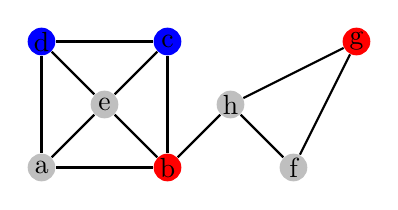
\begin{tikzpicture}[scale=.8,auto,swap]
        %\tikzset{edge/.style = {->,>=latex'}}
        \node[vertex] (a) at (0,0) {a};
        \node[red vertex] (b) at (2,0) {b};
        \node[blue vertex] (c) at (2,2) {c};
        \node[blue vertex] (d) at (0,2) {d};
        \node[vertex] (e) at (1,1) {e};
        \node[vertex] (f) at (4,0) {f};
        \node[red vertex] (g) at (5,2) {g};
        \node[vertex] (h) at (3,1) {h};
        \draw[edge] (a) to (b);
        \draw[edge] (b) to (c);
        \draw[edge] (c) to (d);
        \draw[edge] (d) to (a);
        \draw[edge] (a) to (e);
        \draw[edge] (b) to (e);
        \draw[edge] (c) to (e);
        \draw[edge] (d) to (e);
        \draw[edge] (f) to (g);
        \draw[edge] (f) to (h);
        \draw[edge] (g) to (h);
        \draw[edge] (h) to (b);
      \end{tikzpicture}
    \end{center}

    \item In this graph, the \structure{blue vertices} are 3-edge connected, and the \alert{red vertices} are 1-edge connected;
    \item A {\bf Graph} is k-edge connected if all pairs of vertices are \structure{at least} k-edge connected.
    \end{itemize}
\end{frame}

\begin{frame}{Connected Components}{Edge Connectivity}

  {\large

    \begin{itemize}

    \item {\bf Edge Connectivity} represents the degree of
      {\bf fault tolerance} in a graph.


    \item {\bf Example:} In a communication network, how many
      channels can fail before communication is disrupted?

      \bigskip

    \item Related Concept: \structure{k-vertice connectivity}

      \begin{itemize}
      \item k-vertice connected graph $\implies$ k-edge connected;
      \item \alert{BUT!} k-edge connected $\not\implies$ k-vertice
        connected.
      \end{itemize}

    \item The \structure{complete graph} $K_n$ is n-1 connected.
    \end{itemize}
  }

\end{frame}

\begin{frame}
  \frametitle{Connectivity and Hypercubes}

  {\larger

      \begin{center}
      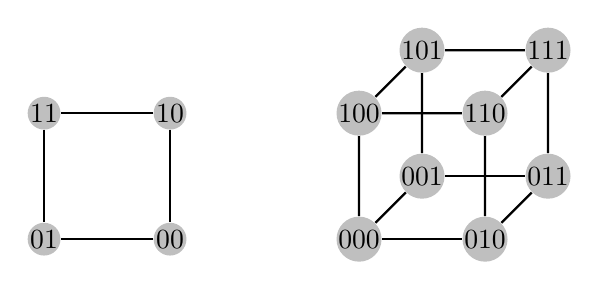
\begin{tikzpicture}[scale=.8,auto,swap]
        %\tikzset{edge/.style = {->,>=latex'}}
        \node[vertex] (00) at (0,0) {00};
        \node[vertex] (01) at (-2,0) {01};
        \node[vertex] (10) at (0,2) {10};
        \node[vertex] (11) at (-2,2) {11};
        \draw[edge] (00) to (10);
        \draw[edge] (10) to (11);
        \draw[edge] (00) to (01);
        \draw[edge] (01) to (11);

        \node[vertex] (000) at (3,0) {000};
        \node[vertex] (010) at (5,0) {010};
        \node[vertex] (100) at (3,2) {100};
        \node[vertex] (110) at (5,2) {110};
        \node[vertex] (001) at (4,1) {001};
        \node[vertex] (011) at (6,1) {011};
        \node[vertex] (101) at (4,3) {101};
        \node[vertex] (111) at (6,3) {111};
        \draw[edge] (000) to (100);
        \draw[edge] (100) to (110);
        \draw[edge] (000) to (010);
        \draw[edge] (010) to (110);
        \draw[edge] (001) to (101);
        \draw[edge] (101) to (111);
        \draw[edge] (001) to (011);
        \draw[edge] (011) to (111);
        \draw[edge] (001) to (000);
        \draw[edge] (111) to (110);
        \draw[edge] (011) to (010);
        \draw[edge] (101) to (100);


      \end{tikzpicture}
    \end{center}

    \begin{itemize}
    \item Consider the $n$-dimensional hypercube $H_n$
    \item $V(H_n) ::= \{0,1\}^n$
    \item $E(H_n) ::= \{(u,v)$ {\bf iff} u and v differ in 1 bit $\}$

    \item $H_n$ is $n$ vertex connected. ($H_n$ has $n^2$ vertices)
    \end{itemize}

  }

\end{frame}

\section{Trees}

\frame{
{Part 3: Trees}

\tableofcontents[currentsection,hideallsubsections, firstsection=1, sections={1-4}]
}


\begin{frame}{Trees and Connectivity}

  {\larger
    \begin{itemize}
    \item \structure{Trees} are connected Graphs with \alert{no cycles}.
    \item Every tree 1-edge connectivity, 1-vertex connectivity.
    \item Chromatic Number = 2 (trees can always be bi-colored)

      \bigskip

    \item Trees come up all the time:
      \begin{columns}
        \column{0.5\textwidth}
        \begin{itemize}
        \item Family Trees;
        \item Search Trees;
        \item Game Trees;
        \item Parse Trees;
        \end{itemize}
        \column{0.5\textwidth}
        \begin{itemize}
        \item Spanning Trees;
        \item Rooted Trees;
        \item Ordered Trees;
        \item Binary Trees;
        \item etc...
        \end{itemize}
      \end{columns}
    \end{itemize}
  }
\end{frame}

\begin{frame}{Trees and Connectivity}

  {\larger
    \begin{itemize}
    \item \structure{Cut Edge}: An edge is a cut edge if
      removing it makes two vertices disconnected.

      \bigskip

    \item {\bf Lemma:} An edge is not a cut edge if it is on a
      cycle.

      \bigskip

    \item A tree is a \structure{connected graph} where
      \structure{every edge is a cut edge}

      \bigskip

    \item This implies that a tree is a connected graph which
      is {\bf\structure{Edge Minimal}}
      \begin{itemize}
      \item A tree has the minimum number of edges necessary to
        connect a set of vertices.
      \end{itemize}
    \end{itemize}
  }
\end{frame}

\begin{frame}
  \frametitle{Tree Coloring}

  {\larger
    \begin{itemize}
    \item A tree is a graph with a \structure{unique path}
      between every pair of vertices.

    \item As a consequence, $\chi(\text{tree}) = 2$

    \item {\bf Constructive Demonstration}

      \begin{columns}
        \column{0.7\textwidth}
        \begin{itemize}
        \item Pick any node in the tree to be the {\bf root}, color
          it ``blue''.
        \item Color nodes ``odd'' length from the root as ``red''
        \item Color nodes ``even'' length from the root as ``blue''
        \item This is the algorithm for 2-coloring on general graphs
        \end{itemize}
        \column{0.3\textwidth}

        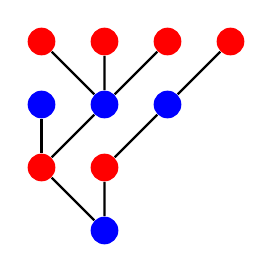
\begin{tikzpicture}[scale=.8,auto,swap]
          %\tikzset{edge/.style = {->,>=latex'}}
          \node[blue vertex] (a) at (1,0) {};
          \node[red vertex] (a1) at (0,1) {};
          \node[red vertex] (b1) at (1,1) {};
          \node[blue vertex] (a2) at (0,2) {};
          \node[blue vertex] (b2) at (1,2) {};
          \node[blue vertex] (c2) at (2,2) {};
          \node[red vertex] (a3) at (0,3) {};
          \node[red vertex] (b3) at (1,3) {};
          \node[red vertex] (c3) at (2,3) {};
          \node[red vertex] (d3) at (3,3) {};
          \draw[edge] (a) to (a1);
          \draw[edge] (a) to (b1);
          \draw[edge] (a1) to (a2);
          \draw[edge] (a1) to (b2);
          \draw[edge] (b1) to (c2);
          \draw[edge] (b2) to (a3);
          \draw[edge] (b2) to (b3);
          \draw[edge] (b2) to (c3);
          \draw[edge] (c2) to (d3);

        \end{tikzpicture}
      \end{columns}

    \end{itemize}



  }
\end{frame}

\subsection{Spanning Trees}

\begin{frame}
  \frametitle{Spanning Trees}

  {\larger

    \begin{itemize}
    \item A \structure{Spanning Subgraph} of G is a subgraph of
      $G$ that has all vertices of $G$ (and some of the edges).
    \item A \structure{Spanning Tree} of G is a spanning graph of
      $G$ that is also a tree.
    \end{itemize}

    \begin{center}
      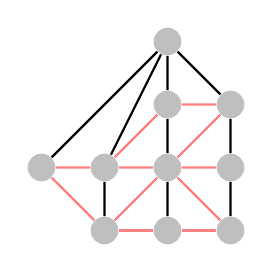
\begin{tikzpicture}[scale=.8,auto,swap]
        %\tikzset{edge/.style = {->,>=latex'}}
        \node[vertex] (a) at (0,1) {};
        \node[vertex] (a1) at (1,0) {};
        \node[vertex] (b1) at (1,1) {};
        \node[vertex] (a2) at (2,0) {};
        \node[vertex] (b2) at (2,1) {};
        \node[vertex] (c2) at (2,2) {};
        \node[vertex] (a3) at (3,0) {};
        \node[vertex] (b3) at (3,1) {};
        \node[vertex] (c3) at (3,2) {};
        \node[vertex] (d3) at (2,3) {};
        \draw[red edge] (a) to (a1);
        \draw[red edge] (a) to (b1);
        \draw[red edge] (a1) to (a2);
        \draw[red edge] (a1) to (b2);
        \draw[red edge] (b1) to (c2);
        \draw[red edge] (b2) to (a3);
        \draw[red edge] (b2) to (b3);
        \draw[red edge] (b2) to (c3);
        \draw[edge] (c2) to (d3);
        \draw[edge] (a) to (d3);
        \draw[edge] (b1) to (d3);
        \draw[edge] (a1) to (b1);
        \draw[red edge] (b1) to (b2);
        \draw[edge] (b2) to (a2);
        \draw[edge] (b2) to (c2);
        \draw[red edge] (a2) to (a3);
        \draw[red edge] (c2) to (c3);
        \draw[edge] (a3) to (b3);
        \draw[edge] (c3) to (d3);
        \draw[edge] (b3) to (c3);
      \end{tikzpicture}
    \end{center}

    \begin{itemize}
    \item One graph can have multiple spanning trees.
    \item Every connected graph has a spanning tree.
    \end{itemize}
  }
\end{frame}

\begin{frame}
  \frametitle{Weighted Spanning Trees}

  {\larger

    The Spanning Tree problem becomes more interesting when we consider
    \structure{weighted edges}.

    \begin{center}
      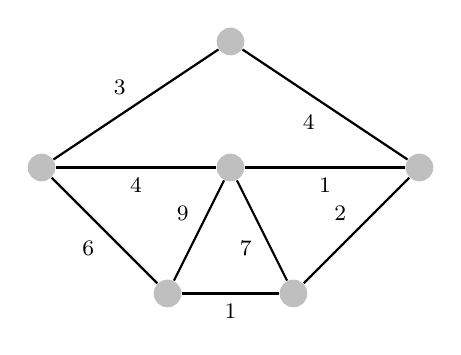
\begin{tikzpicture}[scale=.8,auto,swap]
        %\tikzset{edge/.style = {->,>=latex'}}
        \node[vertex] (a) at (3,5) {};
        \node[vertex] (b) at (0,3) {};
        \node[vertex] (c) at (3,3) {};
        \node[vertex] (d) at (6,3) {};
        \node[vertex] (e) at (2,1) {};
        \node[vertex] (f) at (4,1) {};
        \draw[edge] (a) -- node[weight] {$3$} (b);
        \draw[edge] (a) -- node[weight] {$4$} (d);
        \draw[edge] (b) -- node[weight] {$4$} (c);
        \draw[edge] (c) -- node[weight] {$1$} (d);
        \draw[edge] (b) -- node[weight] {$6$} (e);
        \draw[edge] (c) -- node[weight] {$9$} (e);
        \draw[edge] (c) -- node[weight] {$7$} (f);
        \draw[edge] (d) -- node[weight] {$2$} (f);
        \draw[edge] (e) -- node[weight] {$1$} (f);
      \end{tikzpicture}
    \end{center}

    What is the \structure{minimal cost} structure that
    allows me to connect everything?

  }
\end{frame}

\begin{frame}
  \frametitle{Minimum Spanning Tree Algorithm}

  {\larger
    \begin{center}
      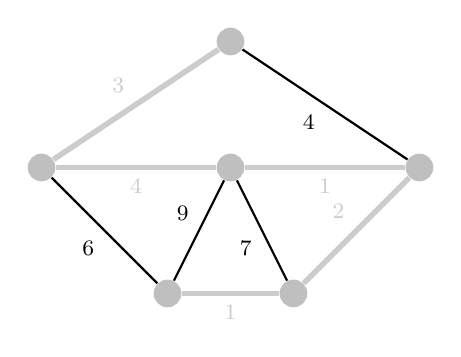
\begin{tikzpicture}[scale=.8,auto,swap]
        %\tikzset{edge/.style = {->,>=latex'}}
        \node[vertex] (a) at (3,5) {};
        \node[vertex] (b) at (0,3) {};
        \node[vertex] (c) at (3,3) {};
        \node[vertex] (d) at (6,3) {};
        \node[vertex] (e) at (2,1) {};
        \node[vertex] (f) at (4,1) {};
        \draw[black edge] (a) -- node[weight] {$3$} (b);
        \draw[edge] (a) -- node[weight] {$4$} (d);
        \draw[black edge] (b) -- node[weight] {$4$} (c);
        \draw[black edge] (c) -- node[weight] {$1$} (d);
        \draw[edge] (b) -- node[weight] {$6$} (e);
        \draw[edge] (c) -- node[weight] {$9$} (e);
        \draw[edge] (c) -- node[weight] {$7$} (f);
        \draw[black edge] (d) -- node[weight] {$2$} (f);
        \draw[black edge] (e) -- node[weight] {$1$} (f);
      \end{tikzpicture}
    \end{center}

    \begin{enumerate}
    \item Start with one arbitrary vertex and add it to the MST.
    \item From all edges connected with the MST, select one with minimum weight;
    \item Add the edge, and vertex, to the MST;
    \item Return to (2)
    \end{enumerate}
  }
\end{frame}

\section{Stable Matching}

\frame{
{Part 4: Stable Matching}

\tableofcontents[currentsection,hideallsubsections, firstsection=1, sections={1-4}]
}

\begin{frame}
  \frametitle{The Stable Marriage Problem}
  \begin{center}
    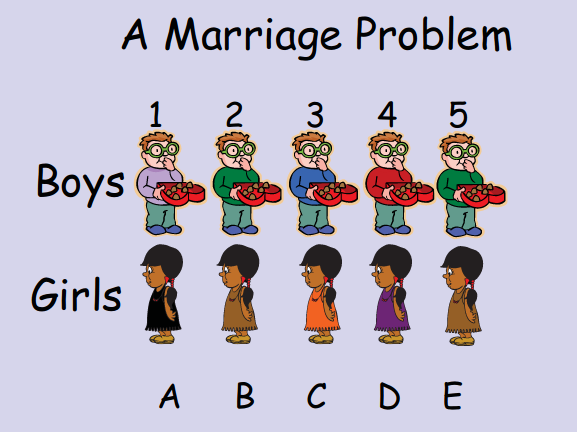
\includegraphics[width=.5\textwidth]{../img/marriage1}\\
    Which boy should marry with which girl?
  \end{center}

\end{frame}

\begin{frame}{The Stable Marriage Problem}{Each boy and girl has a preference list}

  \begin{center}
    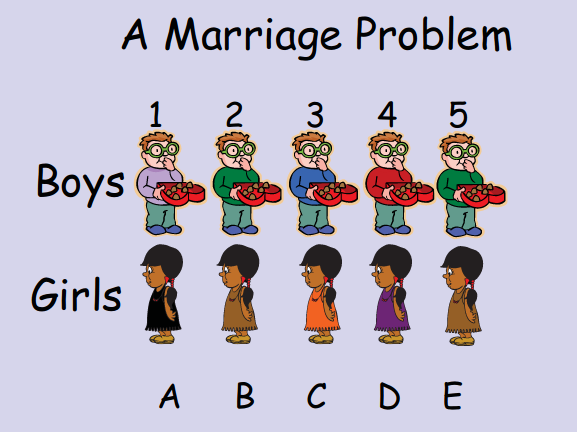
\includegraphics[width=.4\textwidth]{../img/marriage1}
    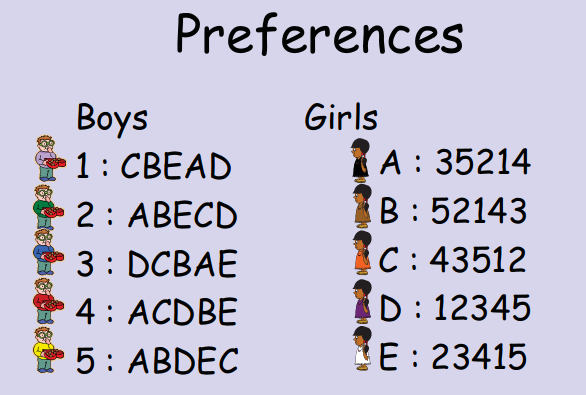
\includegraphics[width=.45\textwidth]{../img/marriage2}
  \end{center}

  Which algorithm do you use to match them?
\end{frame}

\begin{frame}{The "Boy-greedy" algorithm}
  \structure{Boy-greedy algorithm}: Each boy, in order, marries to favorite girl:
  \begin{center}
    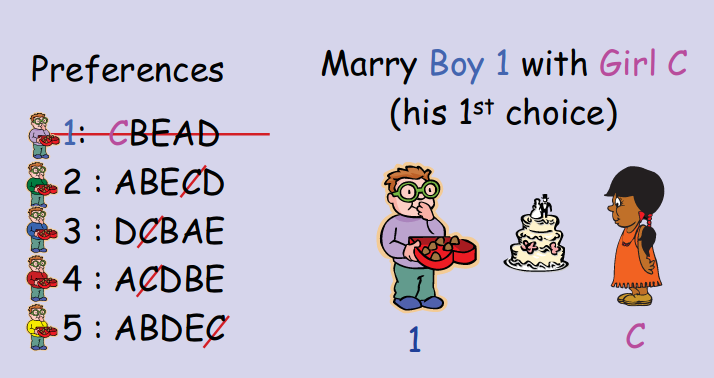
\includegraphics[width=.7\textwidth]{../img/marriage3}
  \end{center}
\end{frame}

\begin{frame}{The "Boy-greedy" Algorithm}

  \structure{Boy-greedy algorithm}: Each boy, in order, marries to favorite girl:
  \begin{center}
    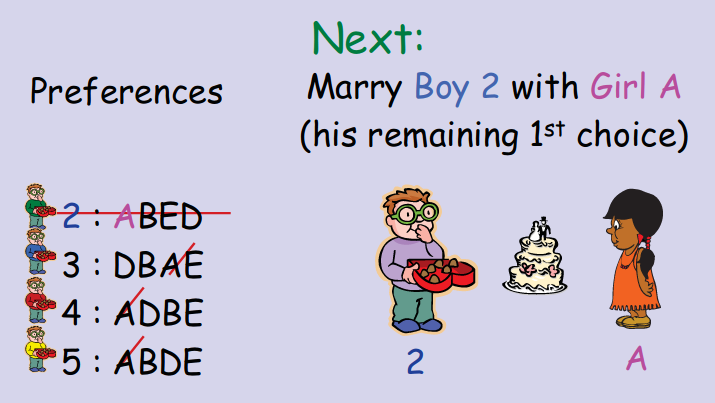
\includegraphics[width=.7\textwidth]{../img/marriage4}
  \end{center}
\end{frame}

\begin{frame}{The "Boy-greedy" Algorithm}{Final Pairings}

  \begin{center}
    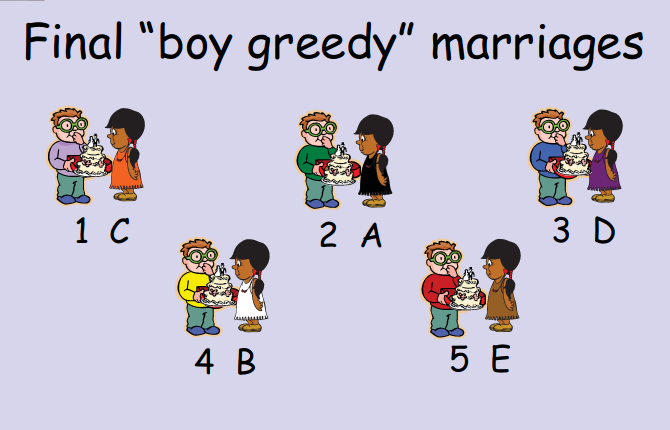
\includegraphics[width=.7\textwidth]{../img/marriage5}
  \end{center}
\end{frame}

\begin{frame}{The "Boy-greedy" Algorithm}{Rogue Couples}
  \begin{center}
    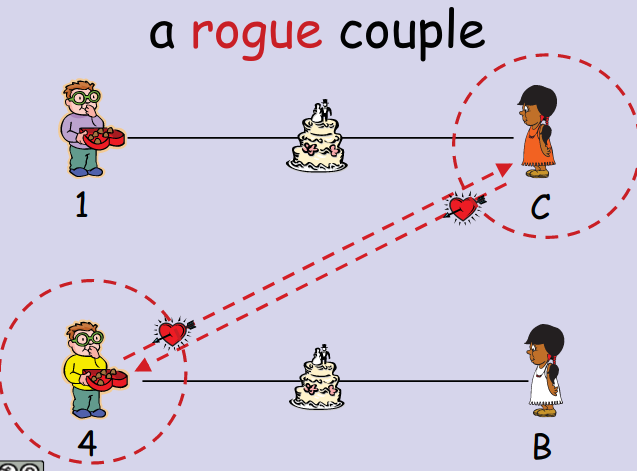
\includegraphics[width=.41\textwidth]{../img/marriage7}
    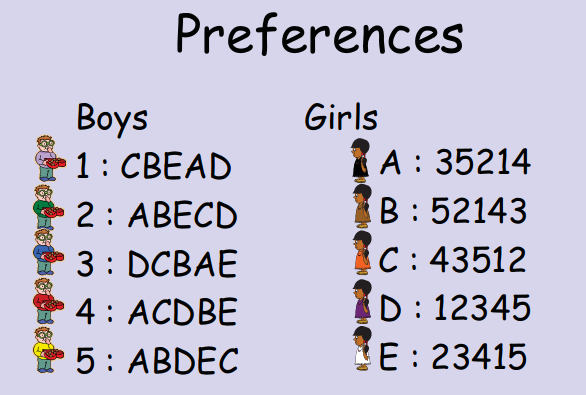
\includegraphics[width=.45\textwidth]{../img/marriage2}
  \end{center}

  \alert{Girl C} likes \structure{Boy 4} better than \structure{Boy 1}. \structure{Boy 4} likes \alert{Girl C} better than \alert{Girl B}.

  Can we find a pairing without rogue couples?
\end{frame}


\begin{frame}{A stable matching}{Using a Girl Greedy algorithm}
  \begin{center}
    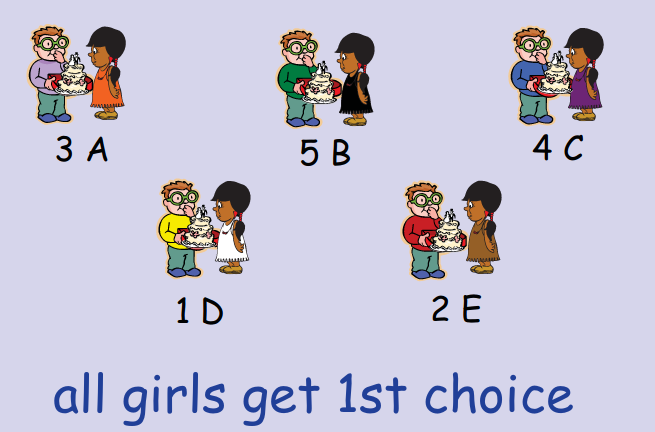
\includegraphics[width=.45\textwidth]{../img/marriage8}
    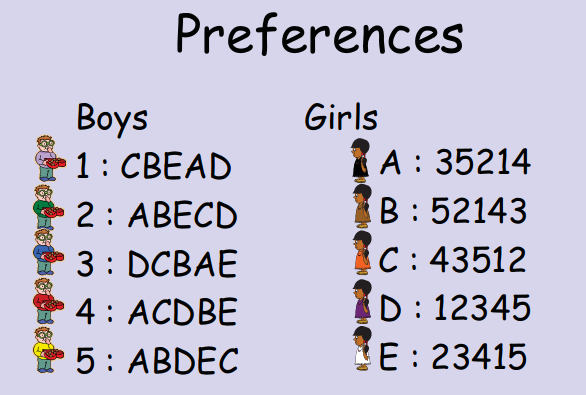
\includegraphics[width=.45\textwidth]{../img/marriage2}
  \end{center}
\end{frame}

\begin{frame}
  \frametitle{Why is the Stable Marriage Problem Important?}

  {\larger
    \begin{itemize}
    \item School Admissions in the US
    \begin{itemize}
      \item Matching school preference and student preference
    \end{itemize}\bigskip


    \item Server/Client Request Matching
    \begin{itemize}
      \item In large webpages, multiple HTTP servers serve the same page for multiple clients;
      \item Servers are matched to clients by geolocation, etc;
    \end{itemize}\bigskip

    \item Etc...
    \end{itemize}
  }
\end{frame}

\subsection{``Mating Ritual'' Algorithm}

\begin{frame}{The ``Mating Ritual'' Algorithm}

    Let us describe an algorithm to {\bf always} find a
    stable matching:\bigskip

    \begin{itemize}
      \item {States}:
      \begin{itemize}
        \item Each boy is proposing to some girl.
        \item Each girl has a list of proposers.
      \end{itemize}
      \item {\bf Start State}: Every boy is proposing to their favorite girl.
    \end{itemize}

    Algorithm:
    \begin{enumerate}
      \item If all girls have $\leq 1$ proposers in their list, they are paired and the algorithm ends;
      \item Any girl with $> 1$ proposers in their list reject all except their favorite proposer;
      \item If a boy is rejected, they propose to the next girl in their list;
      \item Return to (1).
    \end{enumerate}
\end{frame}

\begin{frame}{The Mating Ritual Algorithm}{Example}

  \begin{columns}
    \column{0.45\textwidth}
    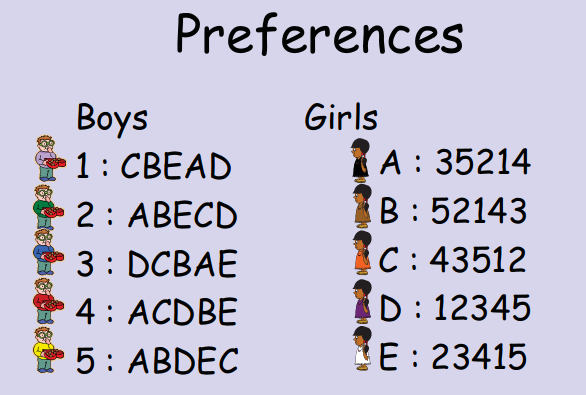
\includegraphics[width=1\textwidth]{../img/marriage2}
    \column{0.55\textwidth}
    {\large
      \begin{itemize}
      \item {\bf iter 1}: No rejections. Proposals:
        \begin{itemize}
        \item A: 2, 4, 5
        \item B:
        \item C: 1
        \item D: 3
        \item E:
        \end{itemize}

      \item {\bf iter 2}: A rejects 2 and 4. Proposals:
        \begin{itemize}
        \item A: 5
        \item B: 2
        \item C: 1, 4
        \item D: 3
        \item E:
        \end{itemize}
      \end{itemize}

    }
  \end{columns}
\end{frame}

\begin{frame}{The Mating Ritual Algorithm}{Example}

  \begin{columns}
    \column{0.45\textwidth}
    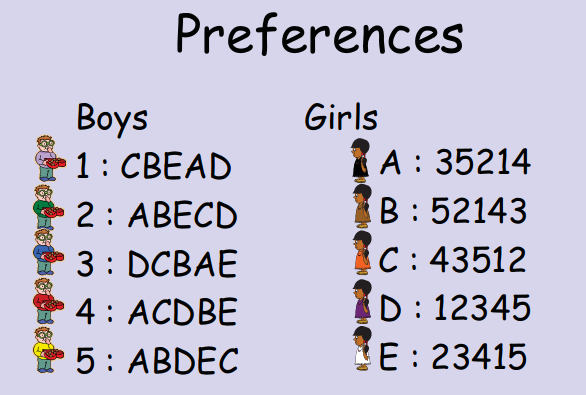
\includegraphics[width=1\textwidth]{../img/marriage2}
    \column{0.55\textwidth}
    {\large
      \begin{itemize}
      \item {\bf iter 3}: C rejects 1. Proposals:
        \begin{itemize}
        \item A: 5
        \item B: 1, 2
        \item C: 4
        \item D: 3
        \item E:
        \end{itemize}

      \item {\bf iter 4}: B rejects 1. Proposals:
        \begin{itemize}
        \item A: 5
        \item B: 2
        \item C: 4
        \item D: 3
        \item E: 1
        \end{itemize}
      \end{itemize}
    }
  \end{columns}
\end{frame}

\begin{frame}{The "Mating Ritual" Algorithm}{Proof of Correctness}

  {\larger
  To proof the correctness of an algorithm, requires that you demonstrate two facts:

    \begin{itemize}
    \item The algorithm stops at some point after the start state;

      \bigskip

    \item The algorithm is correct when it stops;
    \end{itemize}
  }
\end{frame}

\begin{frame}{Proof of Correctness}{The algorithm stops}

  {\larger
    Every day, the \structure{total number} of girls in
    the boy's lists is reduced.

    \bigskip

    \begin{itemize}
      \item Every day, {\bf At least one boy} is rejected by {\bf at least one girl}
      \begin{itemize}
        \item If no boy is rejected, it means that all girls have $\leq 1$ boys in their list
        \item If all girls have $\leq 1$ boys in their list, the algorithm stops;
      \end{itemize}
      \item At some point, every boy's list will have {\bf no girls}:
      \begin{itemize}
        \item A boy with no girls in their list will propose to no one.
        \item If no boys propose, then all girl's lists are empty.
        \item Then the algorithm stops.
      \end{itemize}
    \end{itemize}

    \bigskip

    The total size of "Boy's Lists" is \structure{strictly decreasing}, so the algorithm is guaranteed to stop.
  }
\end{frame}

\begin{frame}
  \frametitle{Proof of Correctness: No rogue couples}

  {\larger

    \begin{itemize}
    \item {\bf Lemma 1}: The rank of a girl's favorite is {\bf weakly
      increasing}\\ Every iteration, the girl rejects a favorite {\bf
      iff} she finds a \structure{better one}.

      \bigskip

    \item {\bf Lemma 2}: The rank of a boy's favorite is {\bf weakly
      decreating}\\ Every iteration, the boy stays with current
      favorite, or is rejected and goes to the next lower one.

    \end{itemize}
  }
\end{frame}

\begin{frame}
  \frametitle{Proof of Correctness: No rogue couples}

  {\larger {\bf Invariant:} If $G_i$ is not on $B_j$ list, she has a
    better curent favorite.

    \bigskip

    \begin{itemize}
      \item At the beginning of the algorithm, $G_i$ is on $B_j$ list;
      \item $G_i$ will reject a boy proposing to her only if a better favorite is also proposing to her;
      \item This implies that a girl's favorite never get worse (lemma 1)
    \end{itemize}
  }
\end{frame}

\begin{frame}
  \frametitle{Proof of Correctness: No rogue couples}

  {\larger

    {\bf Lemma:} When boy $B_i$ is paired, he cannot form a rogue
    couple.

    \bigskip

    {\bf Proof by Cases:}
    \begin{itemize}
    \item {\bf Case 1:} $B_i$ tries to form a rogue couple with
      someone not on his list. However, by \alert{Invariant}, any girl
      not on his list has a better favorite, and no rogue couple is
      possible.

    \item {\bf Case 2:} $B_i$ tries to form a rogue couple with
      someone on his list. However, by \alert{Lemma 2}, $B_i$ always
      propose to the best girl in his list, and no rogue couple is
      possible.
    \end{itemize}

    \bigskip

    {\bf Therefore}, no rogue couple is possible.

  }
\end{frame}

% \begin{frame}
%   \frametitle{Extra Topics}
%
%   {\larger
%
%     Check the class materials for ``Hall's Graphs'', for more
%     information on matching.
%
%   }
%
% \end{frame}


%%%%%%%%%%%%%%%%%%%%%%%%%%%%%%%%%%%%%%%%%%%%%%%%%%%%%%%




\section{Back Matter}
\begin{frame}{Slide Credits}
  These slides were made by Claus Aranha, 2020. You are welcome to copy, re-use and modify this material, following the CC-SA-NC license.
  \bigskip

  These slides are based on "Mathematics For Computer Science (Spring 2015)", by Albert Meyer and Adam Chlipala, MIT OpenCourseWare. \url{https://ocw.mit.edu}.
  \bigskip

  Individual images in some slides might have been made by other
  authors. Please see the following slides for information about these cases.
\end{frame}

\begin{frame}[allowframebreaks]{Image Credits}
  \printnotes
\end{frame}


\end{document}
